\documentclass[12pt]{article}
\usepackage{fancyhdr}
\usepackage[margin=1in]{geometry}
\usepackage{microtype}
\usepackage{lastpage}
%\usepackage{fontspec}
%\setmainfont{Times New Roman}
\usepackage{times}
\usepackage{booktabs}
\usepackage[table]{xcolor}
\usepackage{float}
\usepackage{indentfirst}
\usepackage{url}
\usepackage[pdfborder={0 0 0}]{hyperref}
\usepackage{graphicx}
\usepackage{wrapfig}
\usepackage{caption}
\usepackage{listings}
\usepackage{color}
\usepackage{amsmath}

\date{Fall 2013}
\title{
    \vspace{2in}
    \textmd{\textbf{CS6060- Test 1}}\\
    \vspace{4in}
}
\author{\textbf{Max Thrun}}

\pagestyle{fancy}
\rhead{Max Thrun}
\lhead{CS6060 - Test 1}
\rfoot{Page\ \thepage\ of \protect\pageref{LastPage}}
\cfoot{}
\renewcommand\headrulewidth{0.4pt}
\renewcommand\footrulewidth{0.4pt}

\definecolor{sh_comment}{rgb}{0.12, 0.38, 0.18 } %adjusted, in Eclipse: {0.25, 0.42, 0.30 } = #3F6A4D
\definecolor{sh_keyword}{rgb}{0.37, 0.08, 0.25}  % #5F1441
\definecolor{sh_string}{rgb}{0.06, 0.10, 0.98} % #101AF9
\lstset{
    language=C++,
    xleftmargin=.25in,
    xrightmargin=.25in,
    numbers=left,
    numberstyle=\tiny,
    frame=tb,
    showstringspaces=false,
    captionpos=b,
    stringstyle=\color{sh_string},
    keywordstyle = \color{sh_keyword}\bfseries,
    commentstyle=\color{sh_comment}\itshape,
    basicstyle=\tiny\sffamily,
    %numbersep=-5pt,
    belowskip=\baselineskip,
    aboveskip=\baselineskip
}

\parskip = 0.5\baselineskip
\setlength{\belowcaptionskip}{-\baselineskip}

\captionsetup{font=scriptsize}
\captionsetup{labelfont=bf}

\setlength\parindent{0pt}

\newcommand{\degree}{\ensuremath{^\circ}}

\newcommand{\rotx}[1]{
    \begin{bmatrix}
        1 & 0      & 0       & 0 \\
        0 & \cos#1\degree & -\sin#1\degree & 0 \\
        0 & \sin#1\degree & \cos#1\degree  & 0 \\
        0 & 0      & 0       & 1 \\
    \end{bmatrix}
}

\newcommand{\roty}[1]{
    \begin{bmatrix}
        \cos#1\degree  & 0 & \sin#1\degree & 0 \\
        0       & 1 & 0      & 0 \\
        -\sin#1\degree & 0 & \cos#1\degree & 0 \\
        0       & 0 & 0      & 1 \\
    \end{bmatrix}
}

\newcommand{\rotz}[1]{
    \begin{bmatrix}
        \cos#1\degree & -\sin#1\degree & 0 & 0 \\
        \sin#1\degree & \cos#1\degree  & 0 & 0 \\
        0      & 0       & 1 & 0 \\
        0      & 0       & 0 & 1 \\
    \end{bmatrix}
}

\newcommand{\scale}[3]{
    \begin{bmatrix}
        #1 & 0 & 0 & 0 \\
        0 & #2 & 0 & 0 \\
        0 & 0 & #3 & 0 \\
        0 & 0 & 0 & 1 \\
    \end{bmatrix}
}

\newcommand{\identity}{
    \begin{bmatrix}
        1 & 0 & 0 & 0 \\
        0 & 1 & 0 & 0 \\
        0 & 0 & 1 & 0 \\
        0 & 0 & 0 & 1 \\
    \end{bmatrix}
}
\newcommand{\trans}[3]{
    \begin{bmatrix}
        1 & 0 & 0 & #1 \\
        0 & 1 & 0 & #2 \\
        0 & 0 & 1 & #3 \\
        0 & 0 & 0 & 1 \\
    \end{bmatrix}
}

\newcommand{\mattext}[1]{
    The matrices required to assemble the #1 in its local object space are shown below.
}
\newcommand{\imgtext}[1]{
    The #1 assembly in its local object space is visualized below.
}


\begin{document}
\maketitle
\newpage

\section*{Part A}

    All components in my model are based off a unit cube which is shown below.
    To achieve each shape I simply scale the cube to the appropriate size.  The
    cube extends from \texttt{(0,0,0)} to \texttt{(1,1,1)}. A shader is used to
    draw a grid over the cube with a spacing of 1 unit which allows us to
    visualize the size of the object more easily. Note that while it
    \emph{looks} like multiple cubes are being drawn for each object it is just
    a single stretched cube. Each object is represented by a different color to
    help distinguish them from each other. Note that \emph{all} objects are
    represented by cubes including the lens and baseboard hinge. This was done
    so that we only have to create the vertices for a cube and was deemed
    appropriate as this assignment is more about demonstrating the matrices
    required to build our model. The matrices would remain exactly the same had
    we used proper shapes for all components with the only difference being in
    the vertex buffer.

    \begin{figure}[H]
        \centering
        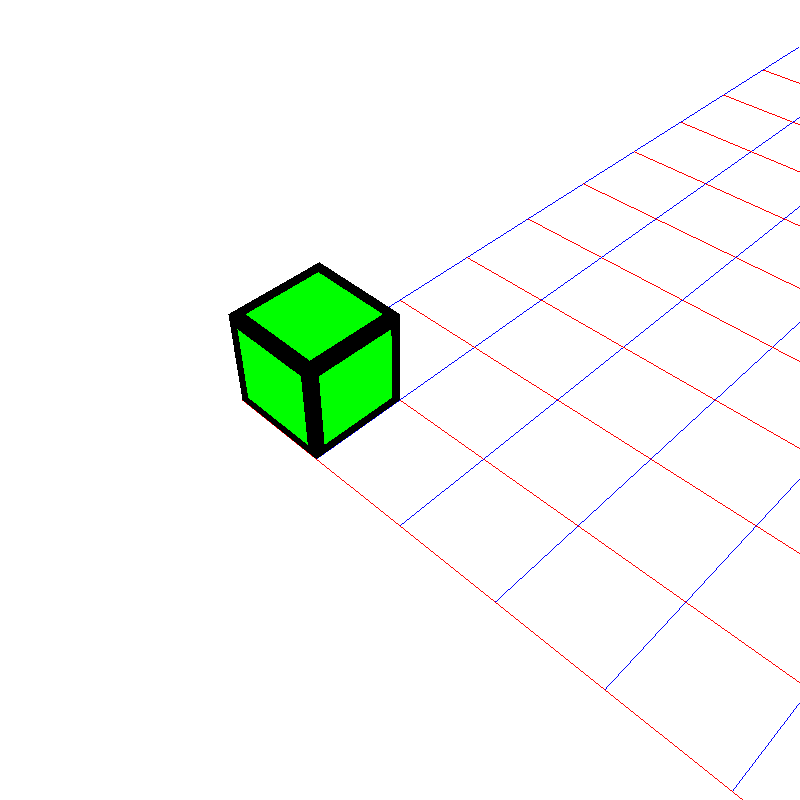
\includegraphics[width=0.5\linewidth]{../images/cube.png}
        \caption{Unit Cube}
    \end{figure}

    The general format for each operation in the following sections is as follows:

    $$ component\_space\_matrix = translation * scale * identity $$

    Note that multiplication is performed right to left in order to ensure that
    we scale before we translate or rotate.

    \vspace{\baselineskip}
    The following sections show the matrices for each component in their
    respective object coordinate spaces.

    \newpage
    \subsection*{Camera}

        \mattext{camera}
        $$
        \begin{aligned}
            cam\_hing\_mcs &= \trans{0}{0}{0} \scale{1}{1}{1} \identity \\
            cam\_body\_mcs &= \trans{1}{-3}{-1.5} \scale{3}{6}{4} \identity \\
            cam\_lens\_mcs &= \trans{1.5}{-4}{-0.5} \scale{2}{1}{2} \identity \\
        \end{aligned}
        $$

        \imgtext{camera}
        \begin{figure}[H]
            \centering
            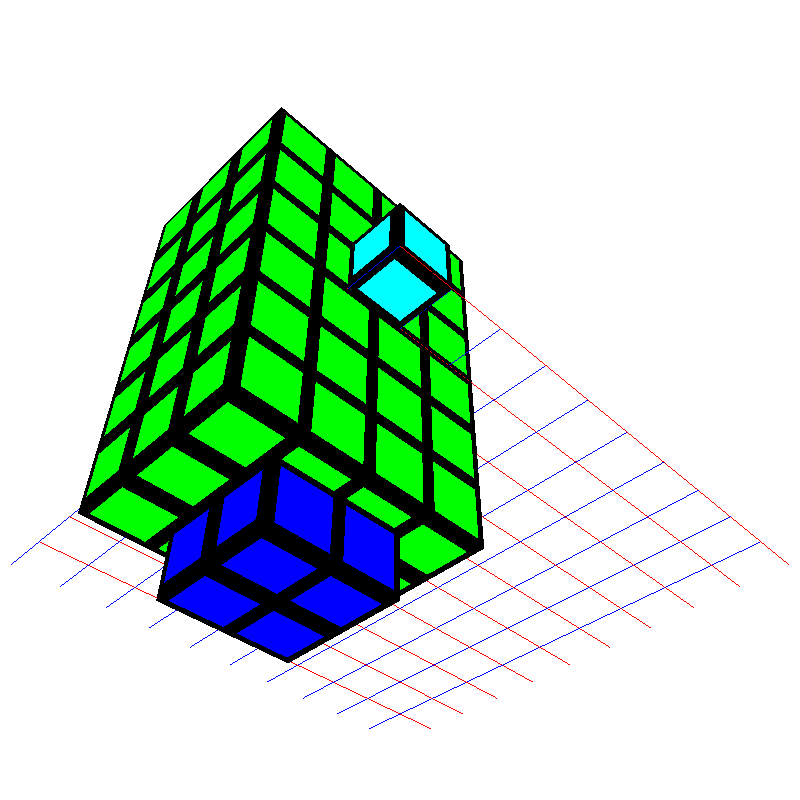
\includegraphics[width=0.75\linewidth]{../images/camera.png}
            \caption{Camera Assembly in MCS space (viewing from bottom)}
        \end{figure}

    \newpage
    \subsection*{Shaft}

        \mattext{shaft}
        $$
        \begin{aligned}
            shaft\_hing\_scs  &=  \trans{0.5}{15}{2} \scale{2}{1}{1} \identity \\
            shaft\_body\_scs  &=  \trans{0}{0}{0} \scale{2}{20}{2} \identity \\
        \end{aligned}
        $$

        \imgtext{shaft}
        \begin{figure}[H]
            \centering
            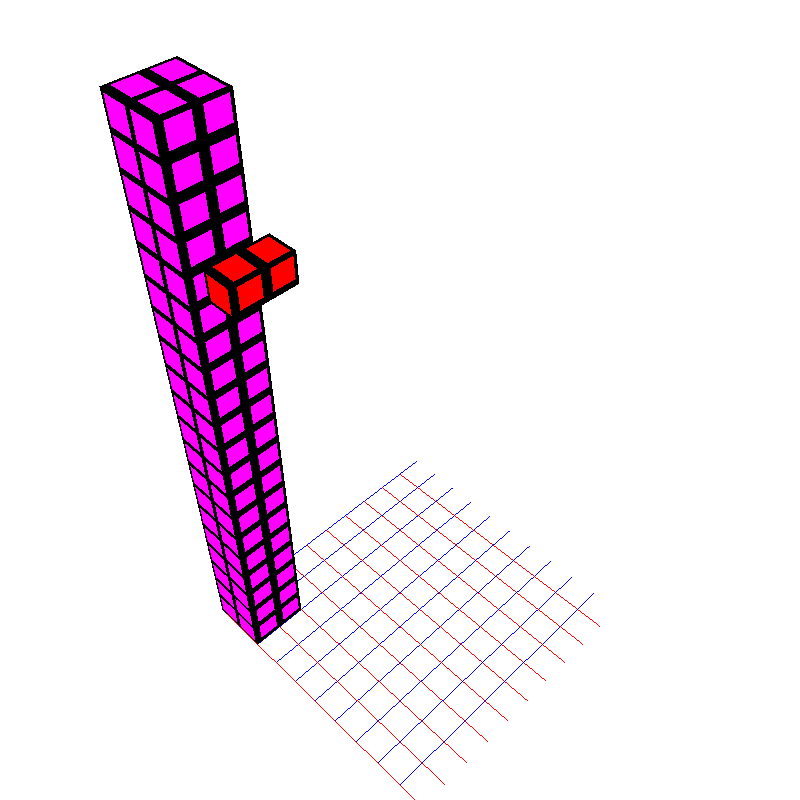
\includegraphics[width=0.75\linewidth]{../images/shaft.png}
            \caption{Shaft Assembly in SCS space}
        \end{figure}

    \newpage
    \subsection*{Baseboard}

        \mattext{baseboard}
        $$
        \begin{aligned}
            base\_hing\_bcs   &=  \trans{3}{2}{2} \scale{6}{3}{6} \identity \\
            base\_body\_bcs   &=  \trans{0}{0}{0} \scale{12}{2}{20} \identity \\
        \end{aligned}
        $$

        \imgtext{baseboard}
        \begin{figure}[H]
            \centering
            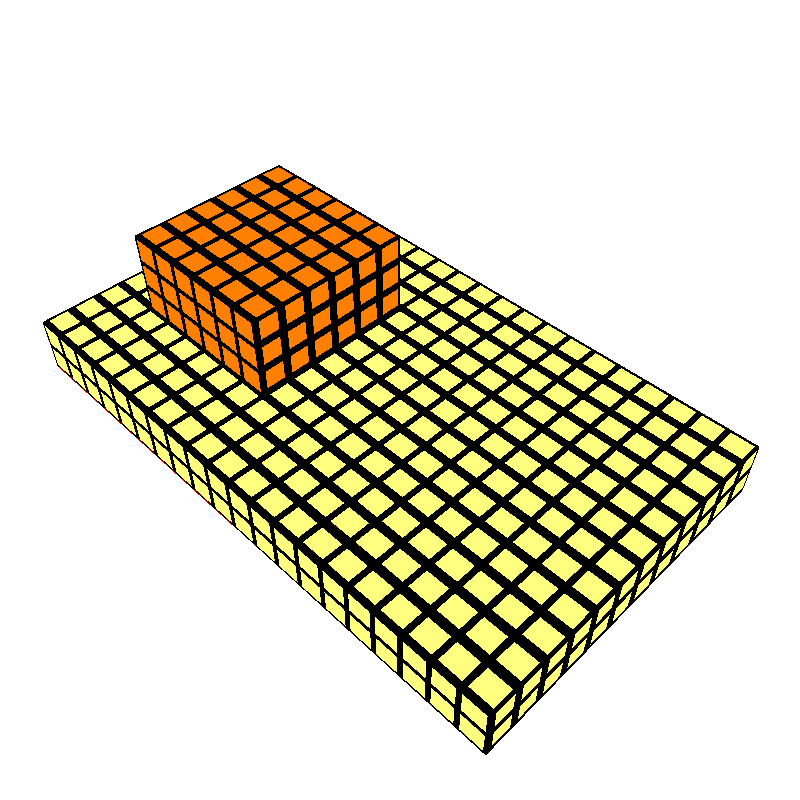
\includegraphics[width=0.75\linewidth]{../images/base.png}
            \caption{Base Assembly in BCS space}
        \end{figure}

    \newpage
    \subsection*{Desk}

        \mattext{desk}
        $$
        \begin{aligned}
            desk\_top     &= \trans{0}{28}{0} \scale{30}{2}{48} \identity \\
            desk\_leg\_1  &= \trans{0}{0}{0} \scale{4}{28}{4} \identity \\
            desk\_leg\_2  &= \trans{26}{0}{0} \scale{4}{28}{4} \identity \\
            desk\_leg\_3  &= \trans{0}{0}{44} \scale{4}{28}{4} \identity \\
            desk\_leg\_4  &= \trans{26}{0}{44} \scale{4}{28}{4} \identity \\
        \end{aligned}
        $$

        \imgtext{desk}
        \begin{figure}[H]
            \centering
            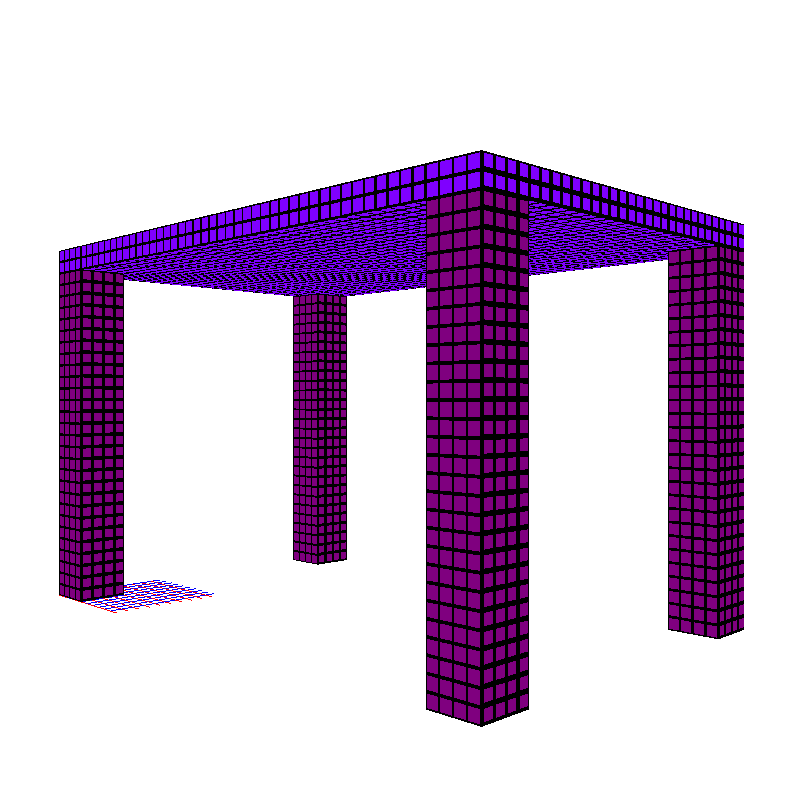
\includegraphics[width=0.5\linewidth]{../images/desk_2.png}
            \caption{Desk Assembly in DCS space}
        \end{figure}

\section*{Part B}

        \mattext{doc-cam}
        $$
        \begin{aligned}
            base\_ocs         &= \identity \\
            base\_hing\_ocs   &=  base\_ocs * base\_hing\_bcs \\
            base\_body\_ocs   &=  base\_ocs * base\_body\_bcs \\
            shaft\_ocs        &= \trans{2}{0}{2} * base\_hing\_ocs * \identity \\
            shaft\_hing\_ocs  &=  shaft\_ocs * shaft\_hing\_scs \\
            shaft\_body\_ocs  &=  shaft\_ocs * shaft\_hing\_scs \\
            cam\_ocs       &= \trans{2}{0}{0} * shaft\_hing\_ocs * \identity \\
            cam\_hing\_ocs &= cam\_ocs * cam\_hing\_mcs \\
            cam\_body\_ocs &= cam\_ocs * cam\_body\_mcs \\
            cam\_lens\_ocs &= cam\_ocs * cam\_lens\_mcs \\
        \end{aligned}
        $$

        \imgtext{doc-cam}
        \begin{figure}[H]
            \begin{minipage}[b]{0.5\linewidth}
                \centering
                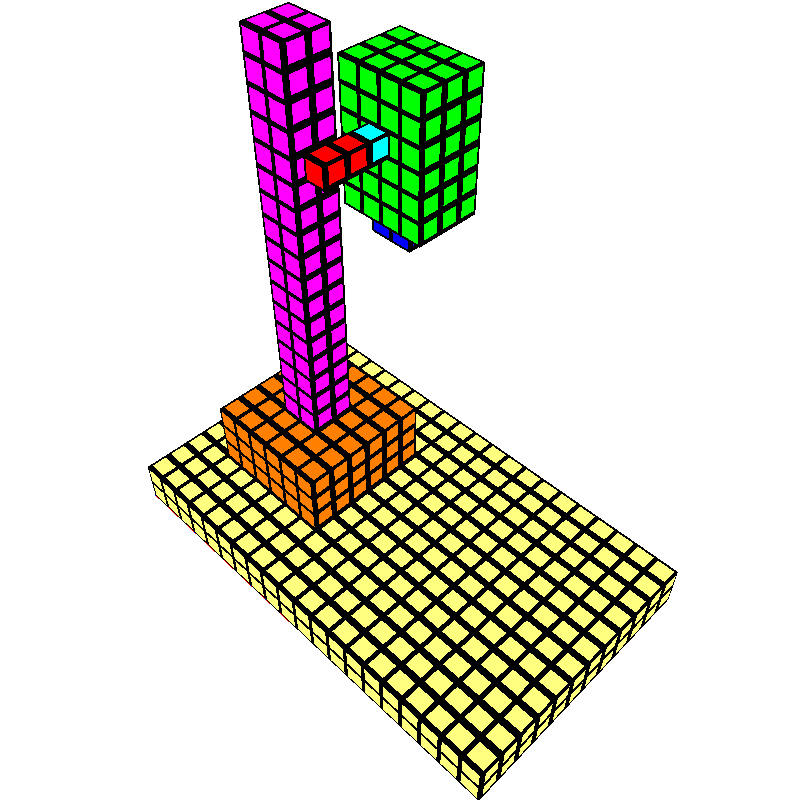
\includegraphics[width=\linewidth]{../images/doccam_1.png}
            \end{minipage}%
            \begin{minipage}[b]{0.5\linewidth}
                \centering
                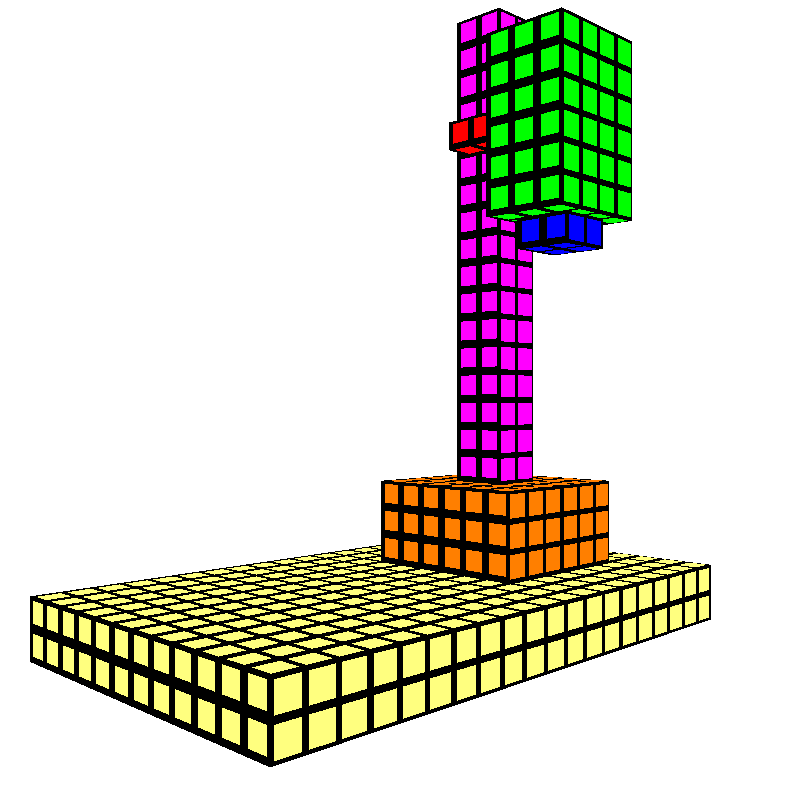
\includegraphics[width=\linewidth]{../images/doccam_2.png}
            \end{minipage}%
            \caption{Doc-cam Assembly in OCS space}
        \end{figure}

\section*{Part C}

        The matrices required to assemble the complete
        model in world space are shown below.

        $$
        \begin{aligned}
            wcs               &= \identity \\
            rcs\_wcs          &= \trans{0}{0}{0} * wcs \\
            dcs\_wcs          &= \trans{0}{0}{0} * rcs\_wcs \\
            ocs\_wcs          &= \trans{9}{30}{16} * dcs\_wcs \\
            desk\_top\_wcs    &= dcs\_wcs * desk\_top\_dcs \\
            desk\_leg\_[1-4]  &= dcs\_wcs * desk\_leg\_[1-4]\_dcs \\
            base\_hing\_wcs   &= ocs\_wcs * base\_hing\_ocs \\
            base\_body\_wcs   &= ocs\_wcs * base\_body\_ocs \\
            shaft\_hing\_wcs  &= ocs\_wcs * shaft\_hing\_ocs \\
            shaft\_body\_wcs  &= ocs\_wcs * shaft\_body\_ocs \\
            cam\_hing\_wcs    &= ocs\_wcs * cam\_hing\_ocs \\
            cam\_body\_wcs    &= ocs\_wcs * cam\_body\_ocs \\
            cam\_lens\_wcs    &= ocs\_wcs * cam\_lens\_ocs \\
        \end{aligned}
        $$

        The completed assembly in world space is visualized below.

        \begin{figure}[H]
            \centering
            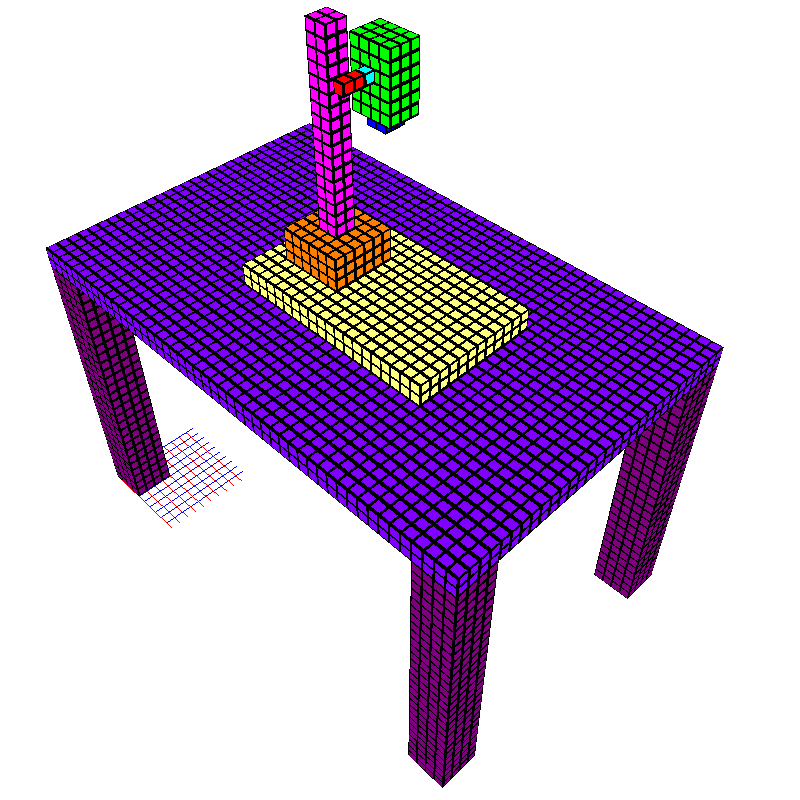
\includegraphics[width=0.25\linewidth]{../images/assembly.png}
            \caption{Full Assembly in WCS space}
        \end{figure}

        \newpage
        Using a simple shader which darkens each face depending on the
        direction of its normal we can achieve a simple `smoothed' version
        which is shown below:

        \begin{figure}[H]
            \centering
            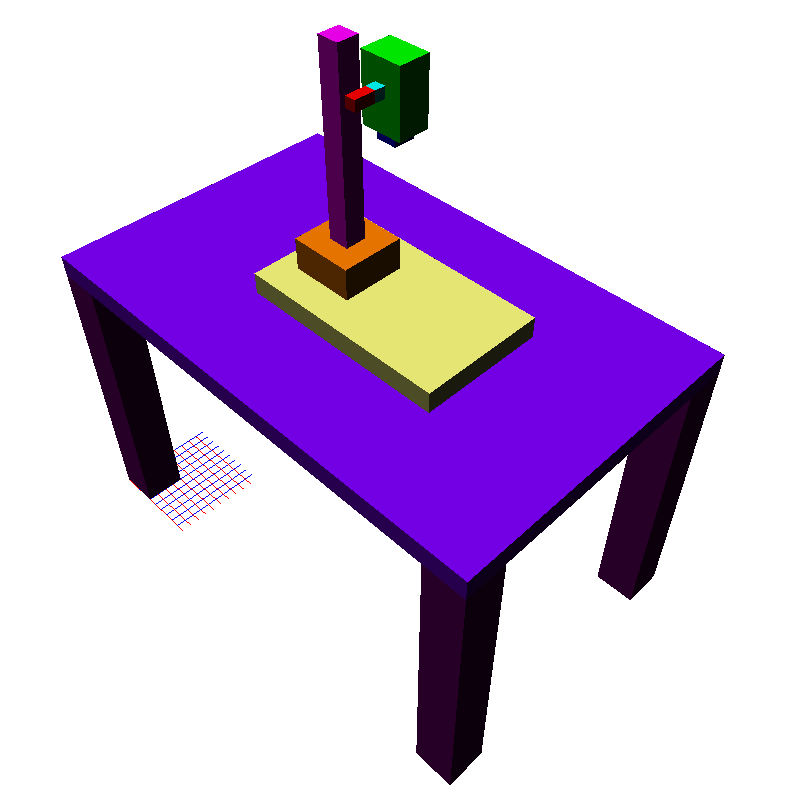
\includegraphics[width=\linewidth]{../images/assembly_smooth.png}
            \caption{Full Assembly in WCS space (smoothed)}
        \end{figure}

        \newpage
        In order to tilt the shaft and camera we simply modify the matrices for
        their respective coordinate systems to include a rotation matrix. The
        matrices shown below are the same as those shown in Part B but with the
        inclusion of a rotation matrix.

        $$
        \begin{aligned}
            shaft\_ocs &= \trans{2}{0}{2} * base\_hing\_ocs * \rotx{30} * \identity \\
            cam\_ocs   &= \trans{2}{0}{0} * shaft\_hing\_ocs * \rotx{-45} * \identity \\
        \end{aligned}
        $$

        \begin{figure}[H]
            \begin{minipage}[b]{0.5\linewidth}
                \centering
                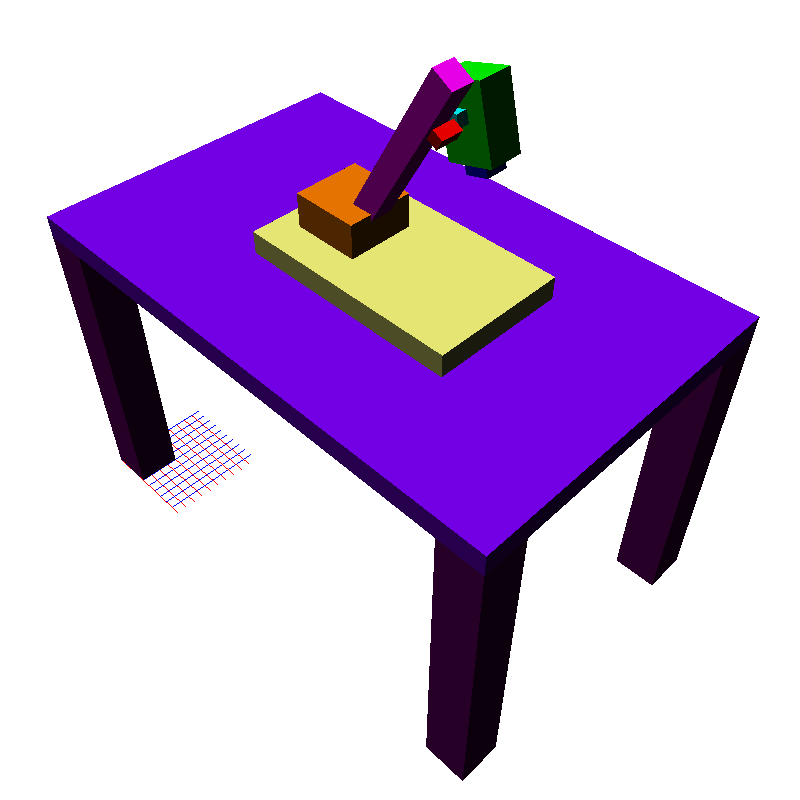
\includegraphics[width=\linewidth]{../images/assembly_smooth_tilt_1.png}
            \end{minipage}%
            \begin{minipage}[b]{0.5\linewidth}
                \centering
                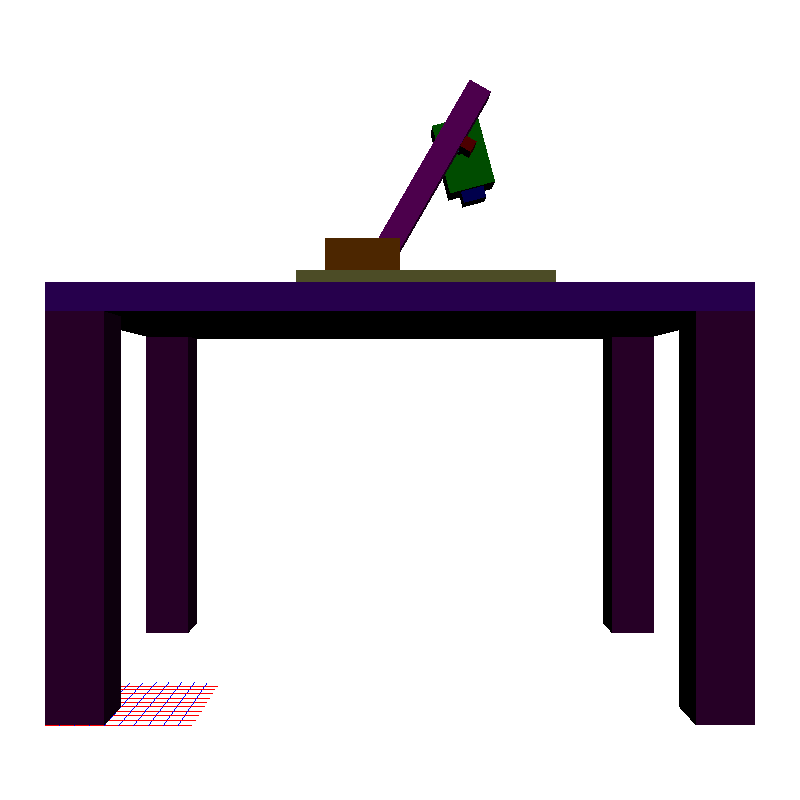
\includegraphics[width=\linewidth]{../images/assembly_smooth_tilt_2.png}
            \end{minipage}
            \caption{Doc-cam Assembly in WCS space with rotated shaft and camera}
        \end{figure}

\newpage
\section*{Part D}
The full source code used to implement this project is shown below. The matrix
definition and operations start on line \texttt{128}.

\lstinputlisting[caption=Main Program]{../main.cpp}
\newpage
\lstinputlisting[caption=Cube Vertex Shader]{../cube_vert.glsl}
\lstinputlisting[caption=Cube Fragment Shader]{../cube_frag.glsl}
\lstinputlisting[caption=Default Vertex Shader]{../default_vert.glsl}
\lstinputlisting[caption=Default Fragment Shader]{../default_frag.glsl}
\end{document}
